\documentclass{article}
\usepackage[utf8]{inputenc}
\usepackage[english]{babel}
\usepackage{graphicx}
\usepackage{float}
\graphicspath{ {} }
\usepackage{mathtools}
\usepackage{amsmath, amsthm, amssymb, amsfonts}
\usepackage{caption}
\usepackage{fancyhdr}
\pagestyle{fancy}
\fancyhf{}
\rhead{Ty Darnell}
\lhead{Homework 2}

% For derivatives
\newcommand{\deriv}[1]{\frac{\mathrm{d}}{\mathrm{d}x} (#1)}

% For partial derivatives
\newcommand{\pderiv}[2]{\frac{\partial}{\partial #1} (#2)}

% Integral dx
\newcommand{\dx}{\mathrm{d}x}
\begin{document}
\begin{flushleft}
\chead{Problems 1-4}
\section*{Problem 1}
\[A_n = \left\{(x,y)|(x-(-1)^n/n)^2+(y)^2<1 \right\}
\]
\[\liminf A_n = \left\{(x,y)|x^2+y^2<1 \right\}
\]
lim inf is contained by the unit circle
\[\limsup A_n=\left\{(x,y)|x^2+y^2\leq 1\right\} -\left\{(0,1),(0,-1) \right\}
\]
lim sup is equal to the unit circle except for the points $(0,1)$ and $(0,-1)$
\begin{figure}[H]
\caption{The center of the circle that contains $A_n$}
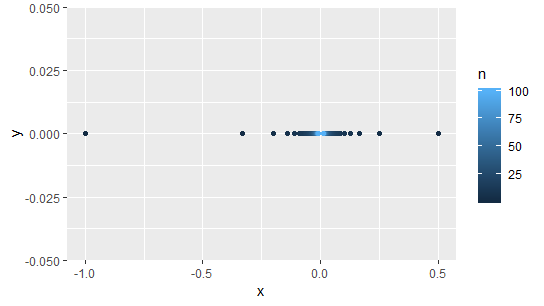
\includegraphics[scale=.85]{pointscircle.png}
\caption{The circle that contains $A_n$}
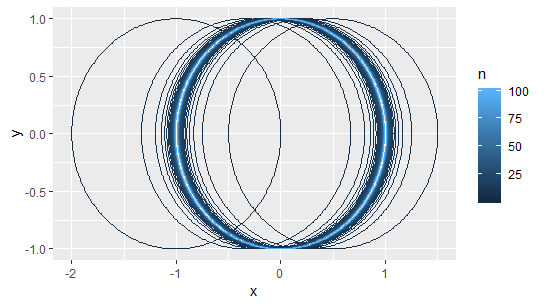
\includegraphics[scale=.85]{circles-100.png}
\end{figure}
\section*{Problem 2}
\begin{align*}
\text{Let } \mathcal{F}&=\left\{A:A \text{ is countable or }A^c \text{ is countable}\right\}\\
\text{We know that } &\emptyset \text{ is countable}\\
\text{Therefore } \emptyset &\in \mathcal{F}\\
\text{Thus } &\mathcal{F} \text{ is nonempty}\\
\text{Let } B_n&=\text{All } A_n \text{ that is countable}\\
\text{Then } B_n &\in \mathcal{F} \text{ and all } {B_n}^c \text{ have countable complements}\\
\text{Which means all }& {B_n}^c \in \mathcal{F}\\
\text{Therefore } \mathcal{F}& \text{ is closed under complementation}\\
&\text{We have two cases:}\\
\textbf{Case 1: }& \text{All } A_n \text{ is countable}\\
\text{Then } \bigcup_{A_n}& \text{ is countable}\\
\text{Therefore } \bigcup_{A_n} &\in \mathcal{F}\\
\text{Thus } \mathcal{F} &\text{ is closed under countable union}\\
\textbf{Case 2: }& \text{At least one } A_n \text{ is not countable}\\
\text{Then }\bigcup_{A_n} \in \mathcal{F} & \iff \left(\bigcup_{A_n}\right)^c \in \mathcal{F} \label{2.1} \tag{1}\\
\text{Then by DeMorgan's Rule }& \left(\bigcup_{A_n}\right)^c = \bigcap_{{A_n}^c}\\
\bigcap_{{A_n}^c} \text{ is countable because at least one }& {A_n}^c \text{ is countable}\\
\text{Thus } \bigcap_{{A_n}^c} &\in \mathcal{F}\\
\text{By } \eqref{2.1} \text{ and DeMorgan's Rule}, \ \bigcup_{A_n} &\in \mathcal{F}\\
\text{Therefore } \mathcal{F} &\text{ is closed under countable union}\\
\text{Conclude } \mathcal{F} \text{ is a }& \sigma \text{ field}
\end{align*}
\section*{Problem 3}
\begin{align*}
\text{Suppose } \chi_1, \chi_2 &\text{ are } \sigma \text{ fields}\\
\text{Let } A&\in \chi_1 \cap \chi_2\\
\text{Then } \chi_1 \cap \chi_2& \text{ is nonempty and }\\
A \in \chi_1 &\text{ and } \chi_2\\
\text{Which means } A^c &\in \chi_1 \text{ and } \chi_2\\
\text{Thus } A^c &\in \chi_1 \cap \chi_2\\
\text{Which means } \chi_1 &\cap \chi_2 \text{ is closed under complementation}\\
\text{Also if } A_1,A_2,\dots &\in \chi_1 \cap \chi_2\\
\text{Then } A_1,A_2,\dots &\in \chi_1, \chi_2\\
\text{Which means } \bigcup \limits_{i=1}^{\infty}A_i &\in \chi_1, \chi_2\\
\text{Thus } \bigcup \limits_{i=1}^{\infty}A_i &\in \chi_1 \cap \chi_2\\
\text{Therefore }  \chi_1 &\cap \chi_2 \text{ is closed under countable unions}\\
\text{Conclude } \chi_1 &\cap \chi_2 \text{ is a } \sigma \text{ field}
\end{align*}
\section*{Problem 4}
\begin{align*}
\text{Suppose } G \text{ is a collection of } &\sigma \text{ fields}\\
\text{Let } G=\chi_1,\chi_2,\dots,\chi_n &\text{ where each } \chi \text{ is a } \sigma \text{ field}\\
\text{We know from problem 3 if:}&\\ \chi_1, \chi_2 \text{ are } \sigma \text{ fields then }& \chi_1 \cap \chi_2 \text{ is a } \sigma \text{ field}\\
\text{Therefore } \forall \ \chi_i \cap \chi_j& \text{ where } \chi_i, \chi_j \in G\\
\text{Then each of these } \chi_i \cap \chi_j &\text{ is also a } \sigma \text{ field}\\
\text{and thus any of these } \chi_i &\cap \chi_j  \text{ interesected}\\
\text{ with another sigma field in } &G \text{ is also a } \sigma \text{ field}\\
\text{Therefore } \bigcap_{\chi \in G} \chi \text{ is also a } &\sigma 
\text{ field}
\end{align*}
\pagebreak
\section*{Problem 5}
\chead{Problems 5-8}
\begin{align*}
\text{Suppose } \chi_1=\left\{\emptyset,A,A^c,\Omega \right\} &\text{ and }
\chi_2=\left\{\emptyset,B,B^c,\Omega \right\}\\
\text{and } \chi_1,\chi_2 &\text{ are } \sigma \text{ fields}\\
\text{Then } \chi_1 \cup \chi_2 &= \left\{\emptyset,A,A^c,B,B^c,\Omega \right\}\\
\text{Since } A \cup B^c &\notin \chi_1 \cup \chi_2\\
\chi_1 \cup \chi_2 &\text{ is not closed under countable unions}\\
\text{Therefore } \chi_1 \cup \chi_2 &\text{ is not a } \sigma \text{ field}
\end{align*}
\section*{Problem 6}
\textbf{Dr. Cai's increasing sequence of sets proof from class}
\begin{align*}
\text{We want to prove if } \left\{E_n\right\}& \text{ is an increasing sequence of sets and }E_n \in \mathcal{A} \text{ then}\\
P(\lim_{n\to \infty}E_n)&=\lim_{n\to \infty}P(E_n)\\
\textbf{Proof:} \text{ Let } F_1=E_1 \text{ and let } &F_j=E_j-E_{j-1} \text{ for } j>1\\
\text{Then } \lim_{n\to \infty} E_n&=\bigcup_{n=1}^{\infty}F_n \text{ and}\\
P(\lim_{n\to \infty} E_n)&=P\left(\bigcup_{n=1}^{\infty}F_n\right)\\
&=\sum \limits_{n=1}^{\infty}P(F_n) \text{ by countable additivity}\\
&=\sum \limits_{n=1}^{\infty}\left[P(E_n)-P(E_n-1) \right]\\
&=\lim_{n\to \infty}P(E_n)\\
\text{Therefore we have proven } P(\lim_{n\to \infty}E_n)&=\lim_{n\to \infty}P(E_n)
\end{align*}
\textbf{Problem 6 Proof}
\begin{align*}
\text{We want to prove } P\left(\lim_{n\to \infty}A_n \right)&=\lim_{n\to \infty}P(A_n)\\
\text{Let } \left\{A_n\right\} \text{ be a decreasing}& \text{ sequence of sets}\\
\text{Which means } A_1 \supset A_2 &\supset \cdots \supset A_n\\
\text{Thus } {A_1}^c \subset {A_2}^c &\subset \cdots \subset {A_n}^c\\
\text{Therefore } \left\{{A_n}^c\right\} \text{ is an} & \text{ increasing sequence of sets}\\
\text{This means } \lim_{n \to \infty} A_n&=\bigcap_{n=1}^{\infty}A_n\\
\text{and } P\left(\lim_{n \to \infty} A_n\right)&=P\left(\bigcap_{n=1}^{\infty}A_n\right) \label{1} \tag{1}\\
\text{Also } \lim_{n \to \infty} {A_n}^c &=\bigcup_{n=1}^{\infty}{A_n}^c\\
\text{and } P\left( \lim_{n \to \infty} {A_n}^c\right) &=P\left(\bigcup_{n=1}^{\infty}{A_n}^c\right) \label{2} \tag{2} \\
\text{From the proof of the increasing}&\text{ sequence of sets from class,}\\
\text{we know that } \eqref{2} &= \lim_{n\to \infty}P({A_n}^c)\\
 \text{Using DeMorgan's Law }& \bigcup_{n=1}^{\infty}{A_n}^c=\left(\bigcap_{n=1}^{\infty}A_n\right)^c \\
 \text{Substituting this into the right side of } &\eqref{2} \text{ we get}\\
 P\left(\left(\bigcap_{n=1}^{\infty} A_n\right)^c\right)&=\lim_{n\to \infty}P({A_n}^c)\\
 1-P\left(\bigcap_{n=1}^{\infty} A_n\right)&=1-\lim_{n\to \infty}P(A_n)\\
 \text{Using algebra we obtain } P\left(\bigcap_{n=1}^{\infty} A_n\right)&=\lim_{n\to \infty}P(A_n) \label{3} \tag{3}\\
 \text{Using } \eqref{1} \text{ and } \eqref{3}& \text{ we can conclude}\\
 P\left(\bigcap_{n=1}^{\infty} A_n\right)&=P\left(\lim_{n \to \infty} A_n\right)=\lim_{n\to \infty}P(A_n)\\
\end{align*}
\section*{Problem 7}
\begin{align*}
P(E \cup F \cup G)&=P[(E \cup F)\cup G]\\
&= P(E \cup F)+P(G)-P[(E \cup F) \cap G]\\
&= P(E \cup F)+P(G)-P([E \cap G] \cup [F \cap G])\\
&=P(E)+P(F)-P(E \cap F)+P(G)-P([E \cap G] \cup [F \cap G])\\
&=P(E)+P(F)-P(E \cap F)+P(G)-P(E\cap G)-P(F \cap G)+P([E\cap G] \cap [F \cap G])\\
&=P(E)+P(F)+P(G)-P(E \cap F)-P(E \cap G)-P(F \cap G)+P(E\cap F \cap G)
\end{align*}
\section*{Problem 8}
\subsection*{a}
\begin{align*}
P(A\cup B)=P(A)+P(B) \quad \text{where } A\in \mathcal{B} \text{ and }& B  \in \mathcal{B} \text{ are disjoint } \text{(Finite additivity)} \label{1} \tag{1}\\
\text{If } A_1,A_2,\dots \in B \text{ are pairwise disjoint, then } P\left(\bigcup_{i=1}^{\infty}A_i \right)&=\sum \limits_{i=1}^{\infty}P(A_i) \quad \text{(Countable additivity)} \label{2} \tag{2}\\
\text{We want to prove } \eqref{2} &\implies \eqref{1}\\
\text{Let } A \text{ and } B& \text{ be disjoint sets}\\
\text{Let }A_1=A, A_2=B, \text{and }& A_i=\emptyset \text{ for } i>2\\
\text{Since } A_i \cap A_j &= \emptyset \quad \forall \ i \neq j\\ 
\text{Then by } \eqref{2} \quad P(A \cup B)=P\left(\bigcup_{i=1}^{\infty}A_i\right) &=\sum \limits_{i=1}^{\infty}P(A_i)\\
\text{Since } P(\emptyset)=0, \quad \sum \limits_{i=1}^{\infty}P(A_i)&=P(A)+P(B)\\
\text{Therefore we have proven } \eqref{2} &\implies \eqref{1}
\end{align*}
\subsection*{b}
\begin{align*}
\lim_{n\to \infty} A_n= \emptyset &\implies \lim_{n\to \infty} P(A_n)=0 \quad \text{(Continuity)} \label{3} \tag{3}\\
\text{We want to prove } \eqref{1} &\text{ and } \eqref{3} \implies \eqref{2}\\
\text{Let } A_1,A_2,\dots &\text{ be pairwise disjoint}\\
\text{Then } P\left(\bigcup_{i=1}^{\infty}A_i \right)&=P\left(\bigcup_{i=1}^{n}A_i \cup \bigcup_{i=n+1}^{\infty}A_i \right)\\
&=P\left(\bigcup_{i=1}^{n}A_i \right)+P\left(\bigcup_{i=n+1}^{\infty}A_i \right) \quad \text{since all } A_i \text{ is disjoint}\\
&=\sum \limits_{i=1}^{n}P(A_i)+P\left(\bigcup_{i=n+1}^{\infty}A_i \right) \quad \text{using finite additivity} \label{4} \tag{4}\\
\text{Let } B_k &= \bigcup_{i=k}^{\infty}A_i\\
\text{Then }B_k \supset B_{k+1} \quad \forall \ k\\
\text{That is } \lim_{k\to \infty}& B_k= \emptyset\\
\text{because }\bigcap_{k=1}^{\infty}B_k&= \bigcap_{k=1}^{\infty}\bigcup_{i=k}^{\infty} A_n=\emptyset \quad \text{since all } A_i \text{ is disjoint}\\
\text{Thus } \limsup A_n &= \emptyset\\
\text{Since } \liminf A_n &\subset \limsup A_n\\
\text{because } \limsup A_n &= \emptyset \text{ and the only thing } \emptyset \text{ can contain is } \emptyset\\
\text{Which means }\liminf A_n &= \emptyset\\
\text{Thus } \limsup A_n&=\liminf A_n=\emptyset\\
\text{Therefore } \lim_{n \to \infty}A_n&=\emptyset\\
\text{That is } \lim_{k\to \infty}& B_k= \emptyset\\
\text{Then from } \eqref{3} \text{ we have } &\lim_{k\to \infty} P(B_k)=0\\
\text{Therefore }  P\left(\bigcup_{i=1}^{\infty}A_i \right)&=\lim_{n\to \infty} P\left(\bigcup_{i=1}^{\infty}A_i \right)\\
&=\lim_{n\to \infty}\left[\sum \limits_{i=1}^{n}P(A_i)+P\left(\bigcup_{i=n+1}^{\infty}A_i \right) \right] \quad \text{from } \eqref{4}\\
\text{Since } \bigcup_{i=n+1}^{\infty}A_i = B_{n+1} &\text{ we can write the above equation as}\\
P\left(\bigcup_{i=1}^{\infty}A_i \right)&=\lim_{n\to \infty}\left[\sum \limits_{i=1}^{n}P(A_i)+P(B_{n+1})\right]\\
\text{Since } \lim_{n\to \infty} &P(B_{n+1})=0 \\
\text{We have } P\left(\bigcup_{i=1}^{\infty}A_1 \right)&=\sum \limits_{i=1}^{\infty}P(A_i)\\
\text{We have shown } &P\left(\bigcup_{i=1}^{\infty}A_i \right)=\sum \limits_{i=1}^{\infty}P(A_i) \quad \text{where } A_i \cap A_j = \emptyset \quad \forall \ i \neq j \\
\text{Therefore we have proven }\eqref{1} &\text{ and } \eqref{3} \implies \eqref{2}
\end{align*}
\section*{Problem 9}
\chead{Problems 9-11}
\subsection*{a}
\begin{align*}
\text{If } P(E)=.9 &\text{ and } P(F)=.8\\
&\text{Then by the inclusion exclusion identity:}\\
P(E \cup F)&= P(E)+P(F)-P(E \cap F)\\
\text{Then } P(E \cup F)&= .9+.8-P(E \cap F)\\
\text{Then } P(E \cup F)&= 1.7-P(E \cap F)\\
\text{Rearranging we get } &P(E \cap F)= 1.7-P(E \cup F)\\
\text{Since } P(E \cup F) &\leq 1\\
\text{and } 1.7-1&=.7\\
P(E \cap F)&\geq .7
\end{align*}
\subsection*{b}
\begin{align*}
\text{We want to show } P(E \cap F)&\geq P(E)+P(F)-1\\
&\text{By the inclusion exclusion identity:}\\
P(E \cup F)&= P(E)+P(F)-P(E \cap F)\\
\text{Rearranging we get } &P(E \cap F)= P(E)+P(F)-P(E \cup F)\\
\text{Since } P(E \cup F) &\leq 1\\
P(E)+P(F)-P(E \cup F)&\geq P(E)+P(F)-1\\
\text{Therefore } P(E \cap F)&\geq P(E)+P(F)-1
\end{align*}
\section*{Problem 10}
\begin{align*}
\text{Proof by induction:}&\\
\forall \ n \in \mathbb{N} &\text{ let } P(n) \text{ be:}\\
P(E_1\cap E_2\cap \cdots\cap E_n)&\geq P(E_1)+P(E_2)+\cdots+P(E_n)-(n-1)\\
\textbf{Basis Step: } P(1)&=P(E_1)\geq P(E_1)-(1-1)\\
\text{Thus } &P(1) \text{ is true}\\
\textbf{Inductive Step: } \text{Let } k&\in \mathbb{N} \text{ and assume }
P(k) \text{ is true:}\\
P(E_1\cap E_2\cap \cdots\cap E_k)&\geq P(E_1)+P(E_2)+\cdots+P(E_k)-(k-1) \label{1}\tag{1}\\
\text{We will prove } &P(k+1) \text{ is true:}\\
P(E_1\cap E_2\cap \cdots\cap E_{k+1})&\geq P(E_1)+P(E_2)+\cdots+P(E_{k+1})-((k+1)-1)\\
P(E_1\cap E_2\cap \cdots\cap E_{k+1})&\geq P(E_1)+P(E_2)+\cdots+P(E_{k+1})-k \label{2} \tag{2}\\
\text{We can rewrite the left side} &\text{ using associativity of intersections}\\
P(E_1\cap E_2\cap \cdots\cap E_{k+1})&=P(E_1\cap E_2\cap \cdots\cap E_{k-1}\cap (E_k\cap E_{k+1}))\\ 
&\geq P(E_1)+\cdots+P(E_{k-1})+P(E_k\cap E_{k+1})-(k-1) \label{3}\tag{3}\\
\text{We know from problem 9 that } &P(E_k\cap E_{k+1})\geq P(E_k)+P(E_{k+1})-1\\
\text{So we can write }& \eqref{3} \text{ as}\\
P(E_1\cap E_2\cap \cdots\cap E_{k+1})&\geq P(E_1)+\cdots+P(E_{k-1})+P(E_k) +P(E_{k+1})-1-(k-1)\\
&\geq P(E_1)+\cdots+P(E_k) +P(E_{k+1})-k \\
&\text{Which is the same as } \eqref{2}\\
&\text{Hence the inductive step has been established}\\
&\text{and by PMI we have proven that:}\\
\forall \ n &\in \mathbb{N} 
\\ P(E_1\cap E_2\cap \cdots\cap E_n)&\geq P(E_1)+P(E_2)+\cdots+P(E_n)-(n-1)
\end{align*}
\section*{Problem 11}
\textbf{a}\quad $\dfrac{3}{5}$\medbreak
\textbf{b} \quad
$\dfrac{3}{5} * \dfrac{2}{5} + \dfrac{2}{5}*\dfrac{3}{4}=\dfrac{3}{5}$\medbreak
\textbf{c}\quad
$\dfrac{3}{5}*\dfrac{2}{4}=\dfrac{3}{10}$

\end{flushleft}
\end{document}
